\documentclass{article}

\usepackage[margin=1in]{geometry}
\usepackage{tikz}
    \tikzstyle{hollow node} = [circle,draw,inner sep=1.5]
    \tikzstyle{solid node}  = [circle,draw,inner sep=1.5,fill=black]
    \usetikzlibrary{calc}
\usepackage{sgame}
    \gamemathtrue
\usepackage[shortlabels]{enumitem}
\usepackage{amsmath}

\author{Damien Prieur}
\title{Problem Set 2 \\ ECON 250}
\date{}

\begin{document}

\maketitle

\section{WATSON 4.2}
Suppose we have a game where $S_1 = {H,L}$ and $S_2 = {X,Y}$.
If player 1 plays $H$, then her payoff is $z$ regardless of player 2's choice of strategy;
player 1's other payoff numbers are $u_1 (L,X) = 0$ and $u_1 (L,Y) = 10$.
You may choose any payoff number you like for player 2 because we will only be concerned with player 1's payoff.
\begin{enumerate}[(a)]
\item Draw the normal form of this game.

\begin{center}
\begin{game}{2}{2}[Player 1][Player 2]
    &    X    &    Y    \\
H   &   z,0   &   z,0   \\
L   &   0,0   &   10,0  \\
\end{game}
\newline
\newline
Note: Player 2 has a payoff of 0 for everything.
\end{center}


\item If player 1's belief is $\theta_2 = (\frac{1}{2},\frac{1}{2})$, what is player 1's expected payoff of playing $H$?
What is his expected payoff of playing $L$?
For what value of $z$ is player 1 indifferent between playing $H$ and $L$.

$$ \text{Expected payoff from H} = \frac{1}{2} \times z + \frac{1}{2} \times z = z $$
$$ \text{Expected payoff from L} = \frac{1}{2} \times 0 + \frac{1}{2} \times 10 = 5 $$
Player 1 is indifferent when
$$\text{Expected payoff from H} = \text{Expected payoff from L} \Rightarrow z = 5$$

\item Suppose $\theta_2 = (\frac{1}{3},\frac{2}{3})$. Find player 1's expected payoff of playing $L$.
$$ \text{Expected payoff from L} = \frac{1}{3} \times 0 + \frac{2}{3} \times 10 = \frac{20}{3} \approx 6.666 $$


\end{enumerate}


\pagebreak
\section{WATSON 6.6}
In the game pictured here, is it ever rational for player 1 to select strategy C? Why?
\begin{center}
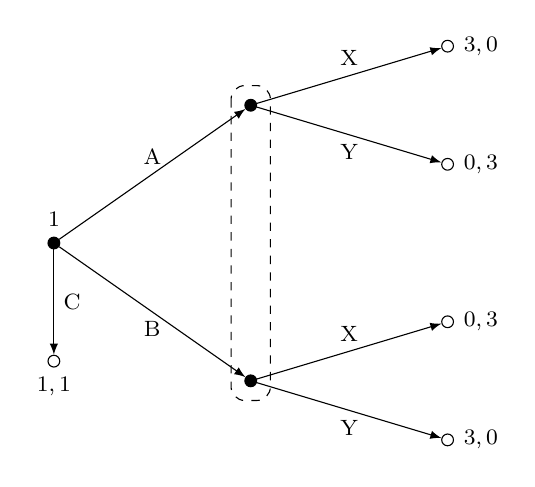
\begin{tikzpicture}[font=\footnotesize,
                    arrow/.style={edge from parent/.style={draw,-latex}},
                    grow' = right
                    ]
\tikzstyle{level 1}=[level distance=25mm, sibling distance=35mm]
\tikzstyle{level 2}=[level distance=25mm, sibling distance=15mm]

    \node(0)[solid node, label=above:{1}]{}
        child[sibling distance=0]{node[draw=none]{} edge from parent[draw=none]}
        child[arrow]{node[solid node]{}
            child[arrow]{node[hollow node, label=right:{$3,0$}]{} edge from parent node[above]{X}}
            child[arrow]{node[hollow node, label=right:{$0,3$}]{} edge from parent node[below]{Y}}
            edge from parent node[above]{A}
        }
        child[arrow]{node[solid node]{}
            child[arrow]{node[hollow node, label=right:{$0,3$}]{} edge from parent node[above]{X}}
            child[arrow]{node[hollow node, label=right:{$3,0$}]{} edge from parent node[below]{Y}}
            edge from parent node[below]{B}
        }
        child[grow'=down, arrow, level distance=15mm]{node[hollow node, label=below:{$1,1$}]{} edge from parent node[right]{C}}
    ;

    \draw[dashed,rounded corners=5]($(0-2)+(-.25,.25)$)rectangle($(0-3)+(.25,-.25)$);

\end{tikzpicture}
\end{center}

It is never rational for player 1 to select strategy C.
If player 1 uses a strategy where they choose between A and B with equal probability then their expected payoff is $\frac{3}{2}$.
This assumes the opponent is also playing rationally as they do not know what our decision is and should also be picking between X and Y equally.
Since the expected payoff is greater with this strategy there is no reason to pick C.

\pagebreak
\section{Game Matrix}
Consider the following game matrix:
\begin{center}
\begin{game}{3}{3}[Player 1][Player 2]
    &    L    &    C    &   R   \\
T   &   3,1   &   0,0   &  4,1  \\
M   &   10,0  &   2,2   &  4,3  \\
B   &   7,6   &   1,2   &  3,1  \\
\end{game}
\end{center}

\begin{enumerate}[(a)]
\item Find all the strictly dominated (pure) strategies for each player.
% strictly dominated strategies: a different strategy is strictly better for that player
\newline
Player 1: B is strictly dominated by M
\newline
Player 2: No strategy is strictly dominated
\item Find all the weakly dominated (pure) strategies for each player.
% weakly dominated strategies: a different strategy is at least as good as the current strategy
\newline
Player 1: T is weakly dominated by M
\newline
Player 2: No strategy is weakly dominated

\item Does the game have a strictly dominant strategy equilibrium?
\newline
Since neither player 1 or 2 has a strictly dominant solution the game does not have a strictly dominant strategy equilibrium.
\end{enumerate}


\pagebreak
\section{Legal Battle}
Two players find themselves in a legal battle over a patent.
The patent is worth 20 for each player, so the winner would receive 20 and the loser 0.
Given the norms of the country they are in, it is common to bribe the judge of a case.
Each player can secretly offer a bribe of 0,9 or 20, and the one whose bribe is largest is awarded the patent.
If both players choose not to bribe, or if the bribes are the same amount, then each has an equal chance of being awarded the patent.
(If a player decides to bribe then he pays the judge regardless of who gets the patent).

\begin{enumerate}[(a)]
\item Derive the game matrix.
\newline
\begin{center}
\begin{game}{3}{3}[Player 1][Player 2]
    &    0    &    9    &   20      \\
0   &  10,10  &  0,11   &   0,0     \\
9   &  11,0   &  1,1    &  -9,0     \\
20  &  0,0    &  0,-9   &  -10,-10  \\
\end{game}
\end{center}
\item Is the game dominance solvable? If so, find the strategy profile surviving IDSDS.
\newline
Since the game is symmetric an argument about strict dominance will apply to both sides.
Bribing \$20 is strictly dominated by bribing \$9 so we can eliminate bribing \$20 for both players which gives us a new game matrix.
\begin{center}
\begin{game}{2}{2}[Player 1][Player 2]
    &    0    &    9    \\
0   &  10,10  &  0,11   \\
9   &  11,0   &  1,1    \\
\end{game}
\end{center}
Now bribing 0 is strictly dominated by bribing 9 so we can eliminate bribing 0.
This game is solvable with IDSDS which reduces to each player bribing 9 with each player having an expected payoff of 1.
\begin{center}
\begin{game}{1}{1}[Player 1][Player 2]
    &    9    \\
9   &  1,1    \\
\end{game}
\end{center}

\end{enumerate}
\end{document}
